%%%%%%%%%%%%%%%%%%%%%%%%%%%%%%%%%%%%%%
%Homaja Marisetty
%CS383 - Team 1
%Design Specs for State and Dimensions
%%%%%%%%%%%%%%%%%%%%%%%%%%%%%%%%%%%%%%

\documentclass[12pt,a4paper]{article}
\usepackage[utf8]{inputenc}
\usepackage{graphicx}
\usepackage[margin=1.0in]{geometry}
\graphicspath{{Users/homanaren/Documents/UI/Spring2017/CS383-Software Engg/sprint2/Final/}}
\begin{document}
\section{Goto State}
The user will be able to move to any state in the frames by clicking on that particular frame.
\subsection{Move Slider}
Scroll bar is set to go to any state at that particular point of time. The slider maximum is set to the maximum number of the frames added.
\section{Dimensions}
This section contains dimensions for main grid and tower grid.
\subsection{Main Grid}
The main grid default dimensions are set to 10*20. User also has a provision to set the dimensions of the main grid area and set the cell color of the grid. Default color is set to black.
\subsection{Tower Grid}
The tower grid default dimensions are set to 5*5. The tower grid is represented with gray color inside the main grid. User can select the tower grid size by pressing the shift key on the start and end rows, columns of the tower grid.
\section{Sample UML Diagrams}
Sample Class and Sequence Diagram for Create grid.
\begin{figure}
\centering
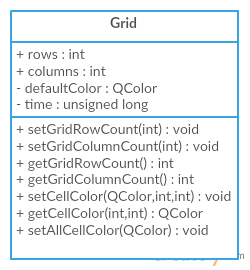
\includegraphics{GridClassDiagram-2.png}
\caption{Grid Class Diagram}
\end{figure}
\begin{figure}
\centering
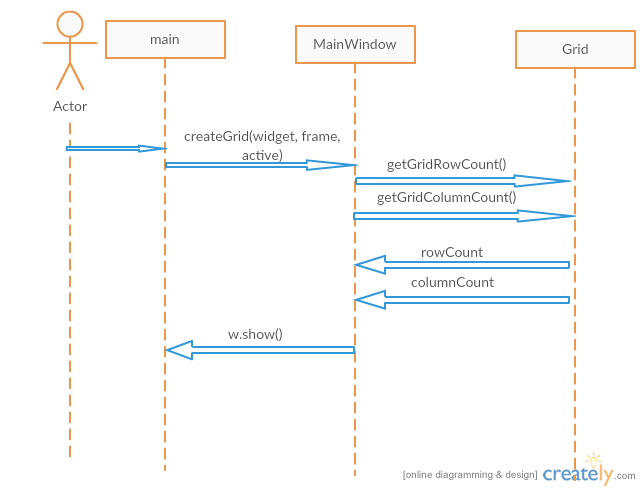
\includegraphics[width = \textwidth]{CreateGridSequenceDiagram.png}
\caption{Sequence Diagram}
\end{figure}
\end{document}
